\documentclass[11pt]{article}

% TVCG Packages
\usepackage{mathptmx}
\usepackage{graphicx}

\usepackage{multirow}
\usepackage{booktabs}
\usepackage{amsmath}
\usepackage{caption}
\usepackage{subcaption}
\usepackage[utf8]{inputenc}
\usepackage{wrapfig}

% Skip paragraphs
%\usepackage{parskip}

\setlength{\parindent}{1em}
\setlength{\parskip}{0.25em}
\renewcommand{\baselinestretch}{1.0}
%\renewcommand{\baselinestretch}{2}

% Change default font to ptsans
%\usepackage[T1]{fontenc}
%\usepackage{paratype}
%\renewcommand{\familydefault}{\sfdefault}
%\linespread{1.00}

% Change default font to Helvetica
\usepackage{helvet}
\renewcommand{\familydefault}{\sfdefault}
%\linespread{1.00}

% Palatino
%\usepackage[sc]{mathpazo} % add possibly `sc` and `osf` options

% Georgia
%\usepackage{fontspec}
%\setmainfont[
%  Ligatures=TeX,
%  BoldFont=Georgia Bold.ttf,
%  ItalicFont=Georgia Italic.ttf,
%  BoldItalicFont=Georgia Bold Italic.ttf
%]{Georgia.ttf}


% Use TitleSec to change headings
%\usepackage{titlesec}
%\titleformat
%  {\section}
%  {\normalfont\rmfamily\Large\bfseries}
%  {\thesection}
%  {1em}
%  {}

% Extra Packages
\usepackage{url}
\usepackage{epstopdf}
\usepackage{arydshln} % For \hdashline in tables
\usepackage{enumitem} % For [noitemsep] in lists

% Coloring author comments
\usepackage{color}
\usepackage[usenames,dvipsnames]{xcolor}
\definecolor{Purple}{rgb}{.75,0,.85}

\newif\ifnotes
\notestrue
\newcommand{\todo}[1]{\ifnotes {\textcolor{Purple}{\bf TODO: #1\ }} \fi}

% if we want to put in page breaks to assess length
\newif\iftestbreaks
\testbreakstrue
\newcommand{\testbreak}{\iftestbreaks\newpage\fi}

% Useful abbreviations
\usepackage{xspace}
\newcommand{\etal}{\emph{et al.}\@\xspace}
\newcommand{\ie}{\emph{i.e.}\xspace}
\newcommand{\eg}{\emph{e.g.}\xspace}
\newcommand{\etc}{\emph{etcetera}\@\xspace}
\newcommand{\etals}{\mbox{\emph{et~al.}'s }}

% TODO NSF CRI / Gleicher commands
\def\naive{na\"{\i}ve}
\def\naively{na\"{\i}vely}

% Droid Sans font
%\usepackage[defaultsans]{droidsans}
%\renewcommand*\familydefault{\sfdefault} %% Only if the base font of the document is to be typewriter style
%\usepackage[T1]{fontenc}
%\linespread{1.1}

%% This turns references into clickable hyperlinks.
\usepackage[bookmarks,backref=true,linkcolor=black]{hyperref} %,colorlinks
\hypersetup{
  pdfauthor = {},
  pdftitle = {},
  pdfsubject = {},
  pdfkeywords = {},
  colorlinks=true,
  linkcolor= black,
  citecolor= black,
  pageanchor=true,
  urlcolor = blue,
  plainpages = false,
  linktocpage
}



\newcommand\figexamples{

  \begin{wrapfigure}{r}{0.5\columnwidth}
  \centering
  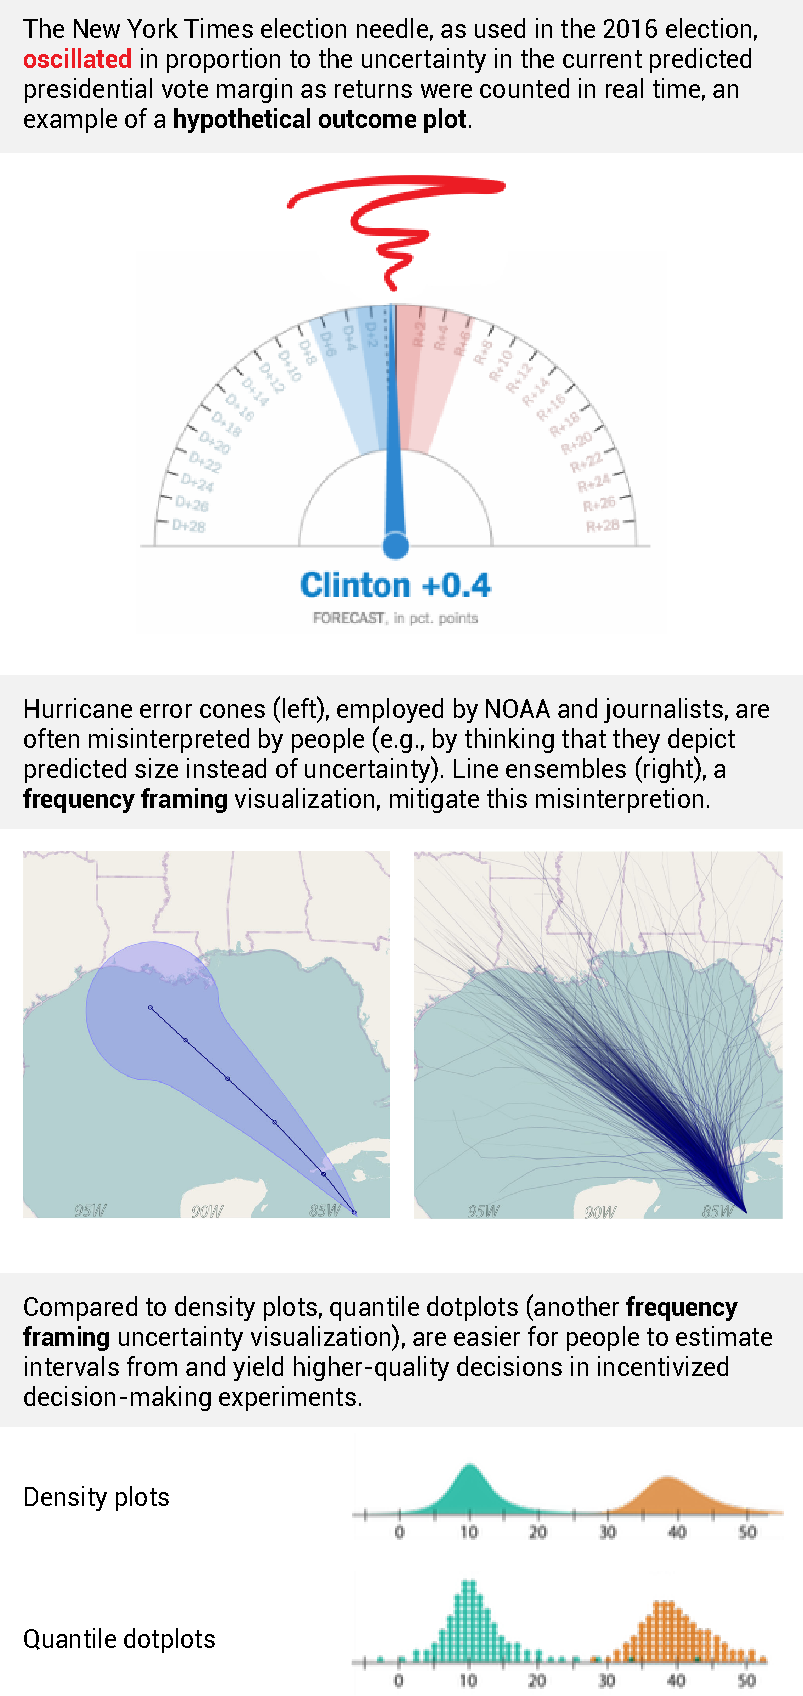
\includegraphics[width=0.5\columnwidth]{img/examples}
  \caption{
    Examples of several uncertainty visualizations one might like to support in a probabilistic grammer of graphics.
  }
  \label{fig:examples}
\end{wrapfigure}

}

\newcommand\figprobgg{

\begin{center}
  \noindent 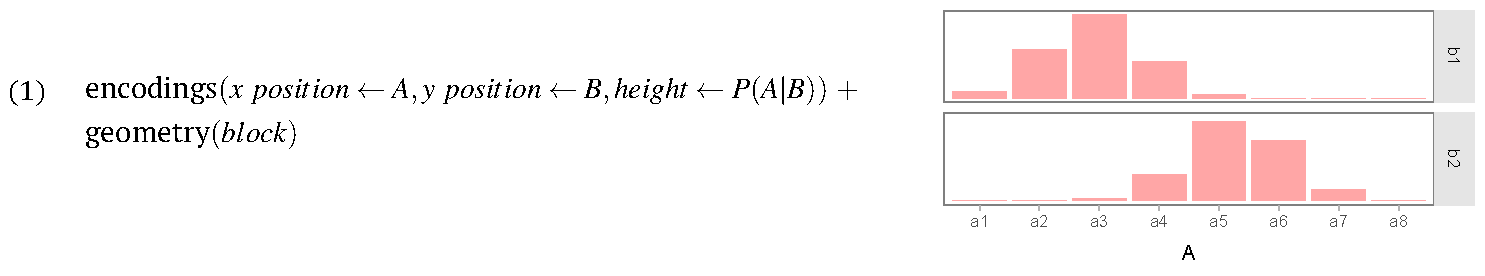
\includegraphics[width=\columnwidth]{img/probgg/prob_gg-1}
  \label{fig:probgg}
\end{center}

\begin{center}
  \noindent 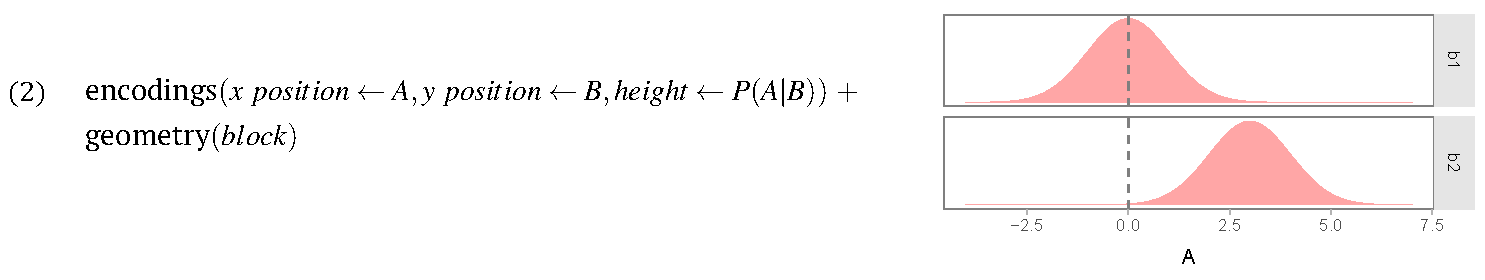
\includegraphics[width=\columnwidth]{img/probgg/prob_gg-2}
  \label{fig:probgg}
\end{center}

\begin{center}
  \noindent 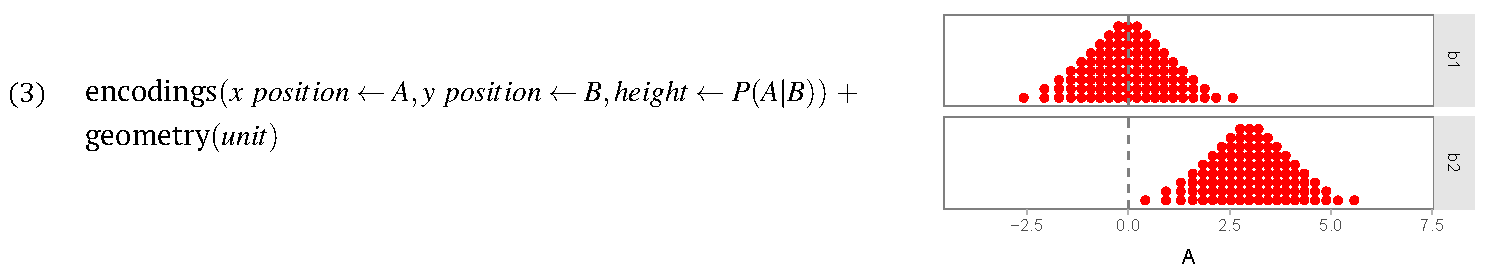
\includegraphics[width=\columnwidth]{img/probgg/prob_gg-3}
  \label{fig:probgg}
\end{center}

}

\newcommand\figboys{

\begin{figure}
  \centering
  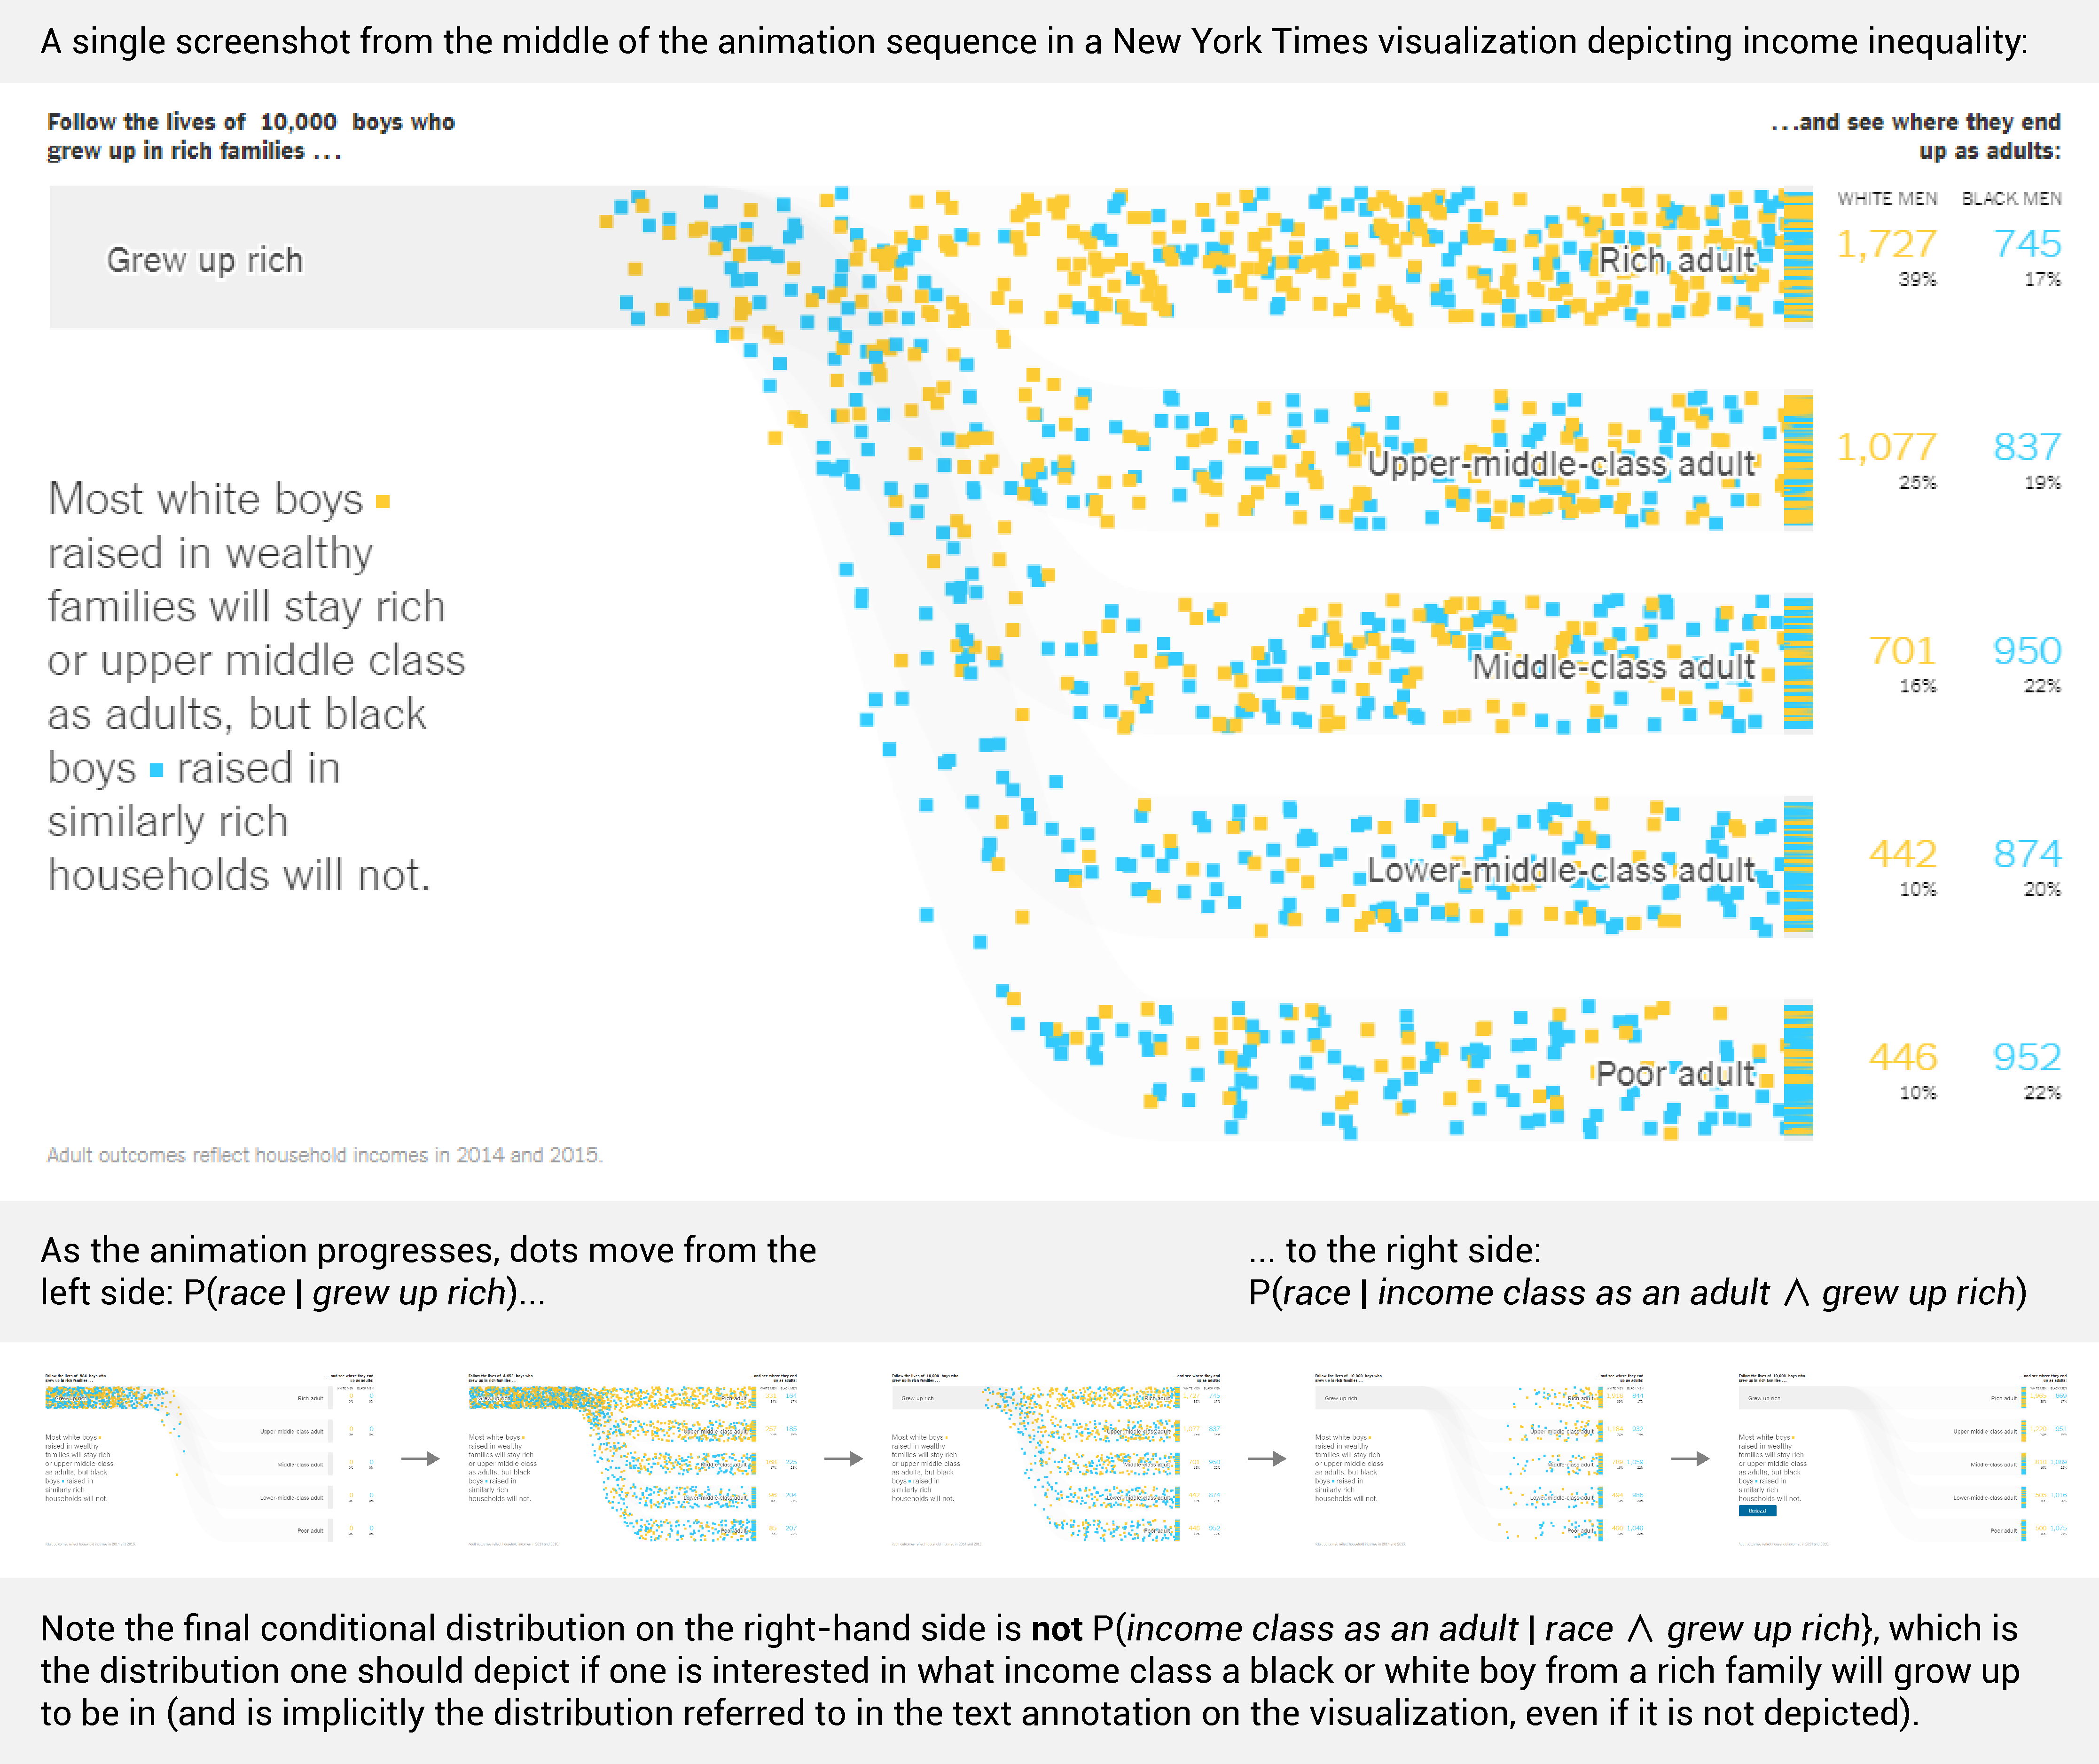
\includegraphics[width=\columnwidth]{img/black-boys/black-boys}
  \caption{
    An example of a professionally-produced probabilistic visualization \cite{badger2018extensive} 
    (\url{https://nyti.ms/2GGpFZw})
    I would both like to be able to support \textbf{and} improve. This visualization falls victim to the \emph{fallacy of the transposed conditional}: by normalizing bar heights on the right-hand 
    side, it depicts $P(race|income~class \wedge grew~up~rich)$ only, so one cannot see 
    $P(income~class | race \wedge grew~up~rich)$: imagine if very few boys of either race who grew up rich ended up in a lower class, then $P(income~class \neq rich | race = black \wedge grew~up~rich)$ would be low even if $P(race = black | income~class \neq rich \wedge grew~up~rich)$ is high. It is worth noting that by reading the numbers in the table to the right it is possible to verify that this is not the case for this particular visualization, but this is difficult to verify from the visualization alone. A probabilistic grammar of graphics would have users explicitly specify the desired distributions, avoiding this error, and would create a similar animation sequence automatically, where this example was custom built in JavaScript.
  }
  \label{fig:boys}
\end{figure}

}





\newcommand\figsystem{

\begin{figure}
  \centering
  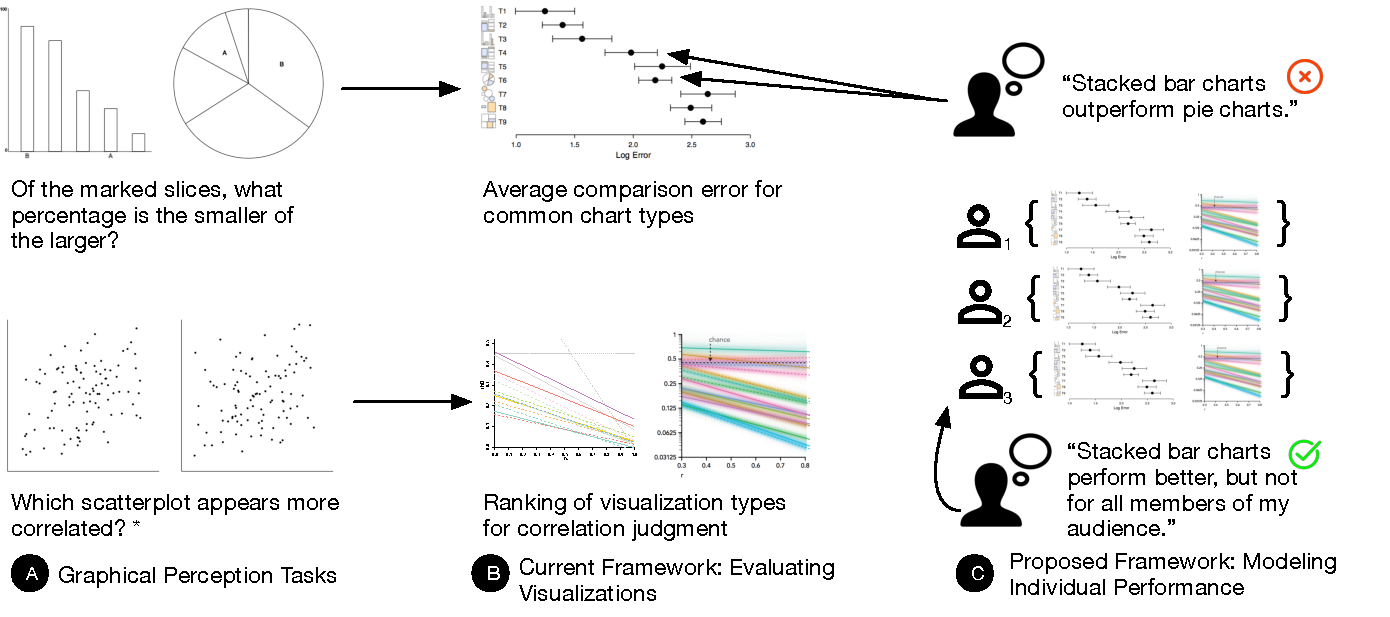
\includegraphics[width=\columnwidth]{old-img/exp-model}
  \caption{
    We propose a new model for graphical perception experiments. A and B illustrate the current model of experiments, where competing visualization designs are evaluated and performance reported for the \emph{average} participant, which by definition leads to overly stringent and possibly incorrect design recommendations in the visualiztion community. C illustrates our proposed framework, in which we \emph{transform} the focus of visualization experiments from evaluating charts to evaluating people, using scalable experiment designs and robust statistical measures. We evaluate our framework using multiple established experiments across diverse participant pools. We evaluate our results through a focused interview study with visualization practitioners. This new model moves to improve and tighten the feedback loop in visualization research, transforming experiments from artifacts to design assets for effective communication through data visualization.
    (*~Can you spot which is most correlated? Our experiments target differences in abilities like this. See the last figure for the answer.)
  }
  \label{fig:system}
\end{figure}

}

\newcommand\figraone{

  \begin{wrapfigure}{r}{0.5\columnwidth}
  \centering
  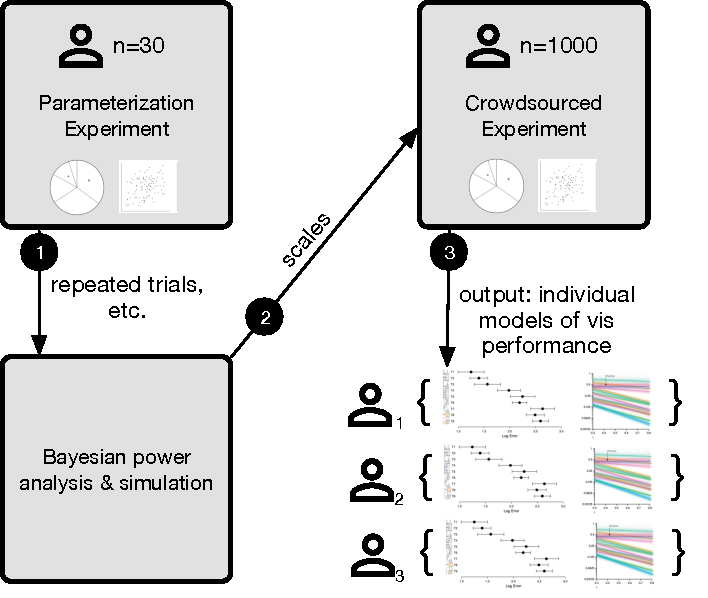
\includegraphics[width=0.48\columnwidth]{old-img/ra1}
  \caption{
    Experiment model for RA1. To evaluate individual differences in visualization performance, we replicate and augment two previously established visualization experiments. We add factors including homogeneous datasets and repeated measures to support between participant comparison and modeling (1). We employ a simulation study (2) to determine parameters for a large crowdsourced experiment with a more diverse population (3).
  }
  \label{fig:ra1}
\end{wrapfigure}

}

\newcommand\figratwo{

  \begin{wrapfigure}{r}{0.5\columnwidth}
  \centering
  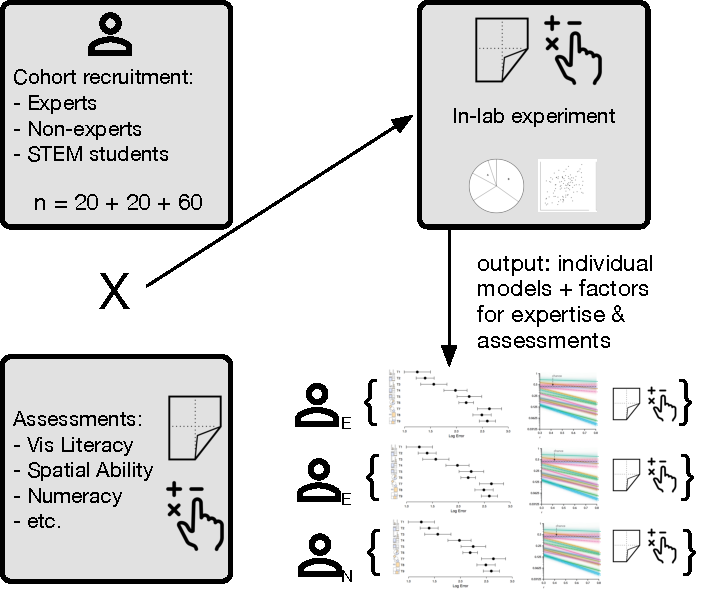
\includegraphics[width=0.48\columnwidth]{old-img/ra2}
  \caption{
    Experiment model for RA2. We explicitly target hypothesized correlates of visualization performance, including expertise, cognitive abilities, and related assessments. We adopt the validated experiment from RA1 as a baseline for an in-lab study, integrate assessments, and extend our robust modeling methodology to evaluate demographics and assessments.
  }
  \label{fig:ra2}
\end{wrapfigure}

}

\newcommand\figrathree{

  \begin{wrapfigure}{r}{0.5\columnwidth}
  \centering
  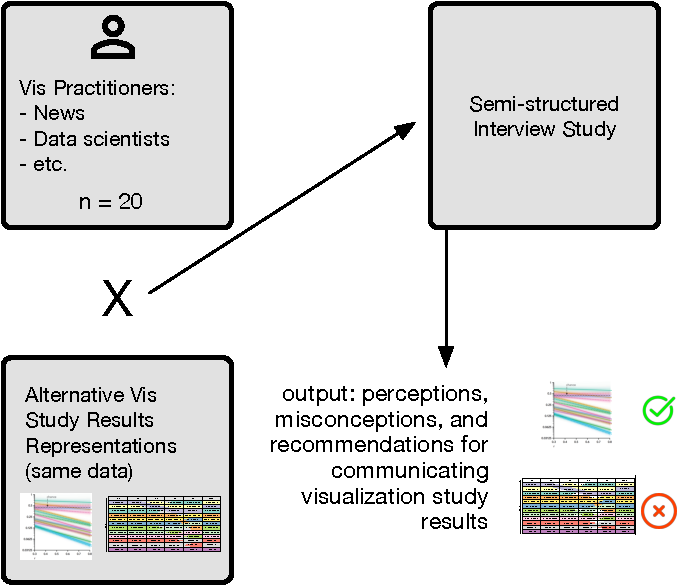
\includegraphics[width=0.48\columnwidth]{old-img/ra3}
  \caption{
    Experiment model for RA3. We challenge longstanding practices in communicating visualization study results. We design alternative representations of study results based on prior work including statistical misconceptions and uncertainty visualization. In an interview study with practitioners, we evaluate how representations shape inferred design guidance that permeates the visualization community.\\
    (*~In Figure \ref{fig:system}, the left scatterplot is most correlated, $r=0.35~v.~0.3$.)
  }
  \label{fig:ra3}
\end{wrapfigure}

}

\newcommand\testtable{

\begin{table}[]
\centering

\begin{tabular}{r c c c c}

& \multicolumn{2}{c}{Our Results} & \multicolumn{2}{c}{Their Results} \\
\multicolumn{1}{l|}{\textbf{Measures}} & \textbf{Exp} & \textbf{Control} & \textbf{Control} & \textbf{Exp} \\ \hline
\multicolumn{1}{l|}{measure A}  & 54.8  & 48.6  & 44  & 33  \\ 
\multicolumn{1}{l|}{measure B}  & 32.2  & 28.8  & 8   & 6   \\ \hdashline
\multicolumn{1}{l|}{measure C} 	& 22.8  & 19.8  & 35  & 26  \\ 

\end{tabular}

\caption{As you can see, we are the best.}
\label{tab:results}
\end{table}

}


%% Packages for proposal writing 
\usepackage[sf,bf,tiny,compact]{titlesec}
% TODO investigate each
\usepackage[labeled]{multibib}
\newcites{m}{References to our work}
\usepackage{float}
\usepackage[rightcaption]{sidecap}
\usepackage[textfont={scriptsize,sf},labelfont={scriptsize,sf,bf}]{caption}
\usepackage[normalem]{ulem}

\titlespacing\section{0pt}{12pt plus 4pt minus 2pt}{0pt plus 2pt minus 2pt}
\titlespacing\subsection{0pt}{12pt plus 4pt minus 2pt}{0pt plus 2pt minus 2pt}
\titlespacing\subsubsection{0pt}{12pt plus 4pt minus 2pt}{0pt plus 2pt minus 2pt}

%% setup for proposal variants
%% for eager variants
\newif\ifeageri
%\eageritrue
\newcommand{\eager}[2] {
\ifeageri #1 \else #2 \fi
}

% this is from the documentation
%\titleformat{\subparagraph}[runin]
%{\normalfont\normalsize\bfseries}{\thesubparagraph}{1em}{}
%\titlespacing*{\subparagraph} {\parindent}{3.25ex plus 1ex minus .2ex}{1em}

% for NIH, we need to use letters for the sections
%% \renewcommand{\thesection}{\Alph{section}}

% if we want to make subsections REALLY tight...
%\titlespacing{\subsubsection}{0pt}{*1}{*0}

% we want to number paragraphs and subpars, but we don't use subsections
\setcounter{secnumdepth}{6}
\def\theparagraph {\thesubsection.\arabic{paragraph}}


% Stephen's layout for NSF proposals. NOT maximal size.
\newlength{\figwidth}
\setlength{\figwidth}{\textwidth}
%\newlength{\captionwidth}
%\setlength{\captionwidth}{1.0\figwidth}

%\setlength{\parindent}{0pt}
%\setlength{\parskip}{1ex}

\setlength{\headheight}{0.0cm}
\setlength{\headsep}{0.0cm}
\setlength{\voffset}{0in}
\setlength{\footskip}{.25in}

%% Set margins and width for NSF (without is thin)
\setlength{\topmargin}{0in}
\setlength{\textheight}{8.9in}
\setlength{\textwidth}{6.5in}
\setlength{\oddsidemargin}{0in}

%% no page numbers for NSF
\pagestyle{empty} \thispagestyle{empty}
% \pagestyle{plain} \thispagestyle{plain}

% TODO try out
\newcommand{\boxit}[2][-10pt]{\vspace{#1}
    \subsubsection*{\framebox{\parbox[t]{\textwidth}{
    \raggedright \rm #2}}}
}

\newenvironment{tight_itemize}     {\begin{itemize}[topsep=0pt, partopsep=0pt]     \itemsep -2pt}  {\end{itemize}}
\newenvironment{tight_enumerate}   {\begin{enumerate}[topsep=0pt, partopsep=0pt]   \itemsep -2pt}  {\end{enumerate}}
\newenvironment{tight_description} {\begin{description}[topsep=0pt, partopsep=0pt] \itemsep -2pt}  {\end{description}}

% use a macro for the subsections of the related work subsection - so
% we can change the formatting as need be
\newcommand{\relatedsection}[1]{\paragraph{#1:}}

% since we use paragraphs without subsections, make sure section does
% the reset
\newcommand{\chuckhack}{}
\newcommand{\mysection}[1]{\section{#1}\setcounter{paragraph}{0}\chuckhack}
\newcommand{\mysubsection}[1]{\subsection{#1}\setcounter{paragraph}{0}\chuckhack}
\newcommand{\mysubsubsection}[1]{\paragraph{#1:}\setcounter{subparagraph}{0}\setcounter{subparagraph}{0}\chuckhack}

% this is from the documentation
%\titleformat{\subparagraph}[runin]
%{\normalfont\normalsize\bfseries}{\thesubparagraph}{1em}{}
%\titlespacing*{\subparagraph} {\parindent}{3.25ex plus 1ex minus .2ex}{1em}

% Change title formatting
\titleformat{\paragraph}[runin]{\sffamily\normalsize\bfseries}
{\theparagraph}{0pt}{~}[~\ ]
\titleformat{\subparagraph}[runin]{\normalfont\normalsize\bfseries}
{\thesubparagraph}{0pt}{~}[~\ ]

\newcommand{\mytitle}{CHS: Small: Developing a Probabilistic Grammar of Graphics\\for Flexible Uncertainty Visualization}

\notestrue
%\notesfalse




\begin{document}

\noindent{\textbf{\mytitle}\\Matthew Kay, University of Michigan\\}

\figexamples

\noindent Journalists and scientists regularly communicate uncertainty information to the general public through visualization. When reporting on high-stakes and uncertain topics ranging from elections to natural disasters, journalists routinely employ visualizations incorporating uncertainty, allowing the public to experience uncertainty to improve understanding and decision-making: \emph{Who will win the next presidential election?} \emph{Should I evacuate in the face of potential flooding?} ``Cones of uncertainty'' are employed by the National Oceanic and Atmospheric Administration to communicate the uncertainty in hurricane path predictions \cite{noaa2014cone}, despite evidence suggesting the uncertainty in these predictions is misinterpreted by the public \cite{ruginski2016nonexpert_hurricane_cones} and the existence of improved alternatives in the literature \cite{padilla2017effects, Mirzargar2014curve_boxplot}. Why does the adoption of more effective uncertainty visualization lag? One reason is that the construction of more sophisticated and effective uncertainty visualizations is more difficult, technically, than the construction of simple, less effective uncertainty visualizations like confidence intervals or prediction cones.

One domain that has seen a more creative approach to uncertainty visualization in journalistic circles is that of election forecasting. During the past several US elections, forecasters at \textit{FiveThirtyEight.com} have directly displayed probability distributions representing their predictions for which party will control the House, Senate, or win the presidential election, often using elaborate interactive visualizations that allow readers to explore many facets of the predictions \cite{noauthor_forecasting_nodate}. In the 2016 presidential election, the \textit{New York Times} created a forecast ``needle'', which displayed the real-time predicted electoral college margin as election returns were being counted \cite{gregor_aisch_live_2016}. The New York Times election needle employed a sophisticated animated uncertainty visualization---the needle jittered in proportion to the prediction's uncertainty---en example of a \emph{hypothetical outcome plot} (HOPs) \cite{hullman2015hops}. HOPs is an approach that has been found to improve lay people's understanding of uncertainty by allowing them to experience uncertainty as natural frequencies, one animated outcome at a time \cite{hullman2015hops, kale2018hypothetical}. 

While more effective, uncertainty visualizations like hypothetical outcome plots are even harder to produce than traditional uncertainty visualizations: The New York Times election needle is a bespoke dynamic JavaScript application created by one of a small number of premier data journalism outfits; its implementation involves correctly handling probability distributions, sampling, and animation, and these aspects are intertwined in the implementation. Besides hypothetical outcome plots, effective---but difficult-to-implement---animated and static uncertainty visualizations exist across many domains, such as transit arrival prediction \citem{kay2016bus, Fernandes2018}, hurricane path prediction \cite{liu2016hurricane, padilla2017effects, Padilla2015, Cox2013hurricane, Mirzargar2014curve_boxplot}, and medical risk communication \cite{Ancker2006}. This technical complexity is not only a barrier to less sophisticated designers (e.g., who do not have access to an in-house team dedicated to implementing visualizations), but is also a barrier to sophisticated designers who might wish to rapidly explore many possible visualization prototypes before settling on a single approach. Currently, therefore, effective uncertainty visualizations are \textbf{difficult to create} and the uncertainty visualization design space is \textbf{costly to explore}.

Various formalizations of information visualization construction into \emph{algebras} \cite{bertin1983semiology, mackinlay1986automating} or \emph{grammars} \cite{wilkinson_grammar_2005} have sought to decrease the technical sophistication users need to create visualizations while simultaneously making it possible to explore a wide range of visualizations easily. The most successful of these have been based on the grammar of graphics \cite{wilkinson_grammar_2005}, which underlies ggplot2 \cite{Wickham2010layered_grammar, wickham2016ggplot2} and Vega-Lite \cite{Satyanarayan2017vegalite}, and the similar VizQL algebra \cite{mackinlay2007show}, which underlies Tableau. These algebras (and the toolkits based on them) are successful because they are not based on a set of predefined template visualizations (too restrictive), nor are they based on a low-level graphics API (unrestrictive---but requiring a large amount of code to create even simple visualizations). Instead, they operate at just the right level of abstraction, one which visualization designers also operate in: they formalize notions of \emph{visual channels} (such as position, length, area, color), \emph{geometries} (such as bars, lines, points, ribbons), and \emph{statistical transformations} (such as means, histograms, kernel density estimators). These primitives can be recombined to create sophisticated visualizations easily, facilitating design exploration. However, none of these grammars formalize the notion of uncertainty or probability, requiring users to recombine statistical transformations and geometries (or worse, to transform input data outside of the visualization framework) in order to create effective uncertainty visualizations (both hypothetical outcome plots \cite{hullman2015hops, kale2018hypothetical} and quantile doplots \cite{kay2016bus, Fernandes2018} would require different preparations of the data in order to be visualized within these frameworks, making design exploration cumbersome).

This work seeks to ask: \emph{How would a grammar of graphics that incorporates uncertainty as a first class entity---a \textbf{probabilistic grammar of graphics}---change how we create uncertainty visualizations?} \emph{Could a simple, consistent probabilistic grammar of graphics be constructed that easily supports a wide range of modern, effective uncertainty visualizations?} \emph{Would a probabilistic grammar of graphics allow designers to more easily explore the space of uncertainty visualizations?} \emph{Would a probabilistic grammar of graphics enable designers to create more correct uncertainty visualizations?} By implementing results of this proposal on top of ggplot2 and Vega-Lite, successful results would lead to improved support for uncertainty visualization in grammar of graphics-based visualization toolkits, making it easier for designers of all expertise levels to adopt effective uncertainty visualization techniques. This would provide substantial improvements to the way that uncertainty and risk are communicated to the public across a range of domains.

\noindent\textbf{Intellectual Merit:} This work addresses the following areas:

\vspace{-0.75em}
\begin{enumerate}[noitemsep]
  \item \textbf{Systematically cataloging existing uncertainty visualizations:}
    I will systematically collect and analyze existing uncertainty visualizations from a variety of sources, including the academic literature and the web. For the academic literature, I will draw upon existing literature reviews of uncertainty visualization and risk visualization \cite{MacEachren1992,Ancker2006,Garcia-Retamero2013,maceachren_visualizing_2005}, including my own work reviewing uncertainty visualization evaluation practices \cite{hullman2018pursuit}. However, many especially expressive examples of uncertainty visualization---particularly those employing sampling-based approaches similar to hypothetical outcome plots---have come from data journalists, as well. Therefore, I expand the scope of existing reviews to include ``best of'' lists of professional information visualizations (\eg Kirk's monthly ``best of'' lists \cite{kirk2018march_best_of_vis}). Finally, I will look at all visualizations produced in 2018 by a small number of well-known, high-quality data journalist teams, such as The New York Times’ Upshot, FiveThirtyEight, and the Guardian. I will collect and classify these visualizations into a taxonomy of uncertainty visualizations.
  \item \textbf{Development of a probabilistic grammar of graphics:}
    Given the visualizations collected in Aim 1, I will develop a specification grammar that encompasses as large a subset of those visualizations as possible while still being grounded in a grammar based on a combination of probability distributions with the grammar of graphics. As the primary goal of this grammar will be to facilitate rapid prototyping, the aim will be to find abstractions that generalize some of the specific instances of charts found while making it easy to quickly try out (or discover) new ways of presenting uncertainty. A secondary goal will be to facilitate the construction of more correct uncertainty visualizations; partly, this will be achieved through grounding the grammar in the specification of probability distributions as probabilistic graphical models, such that if an author wishes to (say) communicate a particular conditional probability, they would specify this in the grammar and the visualization system would determine how to do that. This will allow authors to easily swap out and explore different presentations while maintaining the correctness of the output visualizations.
  \item \textbf{Understanding the expressiveness of the probabilistic grammar of graphics and the correctness of uncertainty visualization in the wild}
    I will re-specify professional, in-the-wild visualizations collected in Aim 1 using the grammar developed in Aim 2. This will enable two goals: first, to determine to the \emph{expressiveness} of the probabilistic grammar of graphics; i.e., to what extent it is capable of generating a large variety of in-the-wild uncertainty visualizations. Second, to assess the correctness of in-the-wild visualizations. Because the grammar will be grounded in formal specification of probability distributions, it will possible to determine if a visualization actually communicates a particular uncertainty correctly. For example, one might ask: if a particular visualization is intended to depict a given conditional probability distribution (e.g., $P(A|B)$), does it? Reasoning about conditional probability can be difficult for people \cite{Gigerenzer1995}, and as described in the Background below, even experts can create visualizations that do not correctly convey the desired probabilities: depending on representation and specification, $P(A|B)$ might not be correctly depicted in a visualization. 
  \item \textbf{Understanding the usability of a probabilistic grammar of graphics}
    I will conduct a user study to assess whether or not visualization authors can rapidly and correctly create uncertainty visualizations using a probabilistic grammar of graphics. I will solicit participants who have been trained in a grammar-of-graphics-based toolkit, such as Vega-Lite \cite{Satyanarayan2017vegalite}. I will have them use either that toolkit or a modified version of the same toolkit to create visualizations of particular distributions, and assess task difficulty and the correctness of created visualizations.
\end{enumerate}

The proposed work will make the creation of sophisticated, easy-to-understand, correct uncertainty visualizations routine for visualization designers, in the same way that the grammar of graphics already facilitates the rapid exploration of visualization design more generally. This work also raises the possibility for future automated visualization design systems to support the creation of verified-correct high-quality uncertainty visualization systems: automated visualization design systems based on grammar of graphics-like formalisms already exist \cite{mackinlay1986automating, moritz2018formalizing}, but do not address uncertainty visualization directly. Provided with a similar formalism for uncertainty visualization, they might.

\noindent \textbf{Broader Impacts of the Proposed Work:} I will directly integrate the output of this research into teaching. I teach a 60-student Professional Master's class in Information Visualization. This class already extensively uses the grammar of graphics to teach students how to reason about and construct effective visualizations, and students are taught both the Vega-Lite \cite{Satyanarayan2017vegalite} and Tableau \cite{mackinlay2007show} visualization toolkits. I also teach a module on uncertainty visualization in that class. I will integrate the probabilistic grammar of graphics into this curriculum, enhancing students' understanding of uncertainty visualization. The University of Michigan School of Information is also launching an online Master's degree as a series of Massic Open Online Courses (MOOCs), one of these will be a course on uncertainty visualization, which I will incorporate content from the results of this proposal into.

I will also build out probabilistic extensions to both Vega-Lite \cite{Satyanarayan2017vegalite} and ggplot2 \cite{wickham2016ggplot2}, popular grammar of graphics toolkits. I have a track record of creating and maintaining open source tools, including tidybayes \cite{kay2017tidybayes}, an R package for visualizing Bayesian regression output in R; this package receives over 1000 downloads per month. With widely available methods for quickly building and prototyping uncertainty visualizations built on top of popular visualization toolkits, more effective uncertainty visualizations can proliferate. This will make the construction of correct, effective uncertainty visualization routine, which will in turn help the public make better decisions under uncertainty all the way from domains like transit decision-making \cite{kay2016bus,Fernandes2018} to medical decision-making \cite{Ancker2006} to decision-making during natural disasters \cite{padilla2017effects, Cox2013hurricane, Mirzargar2014curve_boxplot} to decisions during elections \cite{gregor_aisch_live_2016}.



\section{Background and Related Work}

\noindent To put the proposed research in context, here I provide a discussion of the most related work in uncertainty visualization and the construction of visualizations through the grammar of graphics.

\noindent \textbf{Uncertainty Visualization}: A starting point for distinguishing uncertainty visualization types is whether those visualizations use \emph{intrinsic} or \emph{extrinsic} representations of uncertainty \cite{kay2016bus}. A common \emph{extrinsic} representation is an annotation such as a confidence interval or confidence band. Such representations are notoriously difficult for people to correctly interpret \cite{belia2005ci}, and often underperform other \emph{intrinsic} representations, such as hypothetical outcome plots \cite{hullman2015hops, kale2018hypothetical}, quantile dotplots \cite{kay2016bus, Fernandes2018}, or line ensembles \cite{padilla2017effects}. Intrinsic representations may vary from more abstract representations, such as densities \cite{Ibrekk1987}, to \emph{frequency framing} approaches, in which discrete outcomes are shown. 

Frequency framing approaches are motivated by literature suggesting that people better reason about Bayesian probability when presented with probabilities as natural frequencies instead of abstract probabilities \cite{Gigerenzer1995} (\eg \emph{7 out of 10} instead of \emph{70\%}). The classic example of a frequency framing approach is an \emph{icon array} \cite{Ancker2006}, which displays uncertainty in a categorical variable using a matrix of possible outcomes (such as dots or icons of individuals) and which is commonly used in medical risk communication. I extended the icon array approach to apply to continuous random variables by introducing \emph{quantile dotplots}, which improve probability estimation and decision-making over intervals or densities \cite{kay2016bus, kale2018hypothetical}. Hullman \etal introduced an animated frequency framing uncertainty visualization, hypothetical outcome plots (HOPs), which also improve performance over common static and non-frequency framing approaches \cite{hullman2015hops,kale2018hypothetical}. Building on these recent advances in effective, \emph{intrinsic} uncertainty visualizations, an important goal of the proposed work is to support intrinsic, frequency-framing uncertainty visualization approaches in particular, as evidence increasingly suggest these approaches better align with how people reason about uncertainty. At the same time, correctly constructing frequency framing uncertainty visualizations is often technically more difficult than simple extrinsic displays, like confidence intervals.

\noindent \textbf{The Grammar of Graphics}: The Grammar of Graphics is a systematic way of describing the elements in a visualization, such as data, geometries, visual encodings,\footnote{I use \emph{visual encodings} in place of \emph{aesthetics}---as they are called in ggplot2---to be more consistent with terminology elsewhere in the visualization literature.} statistical transformations, and scales \cite{wilkinson_grammar_2005, Wickham2010layered_grammar, wickham2016ggplot2}. As an example, a simple scatterplot of variable $A$ against variable $B$ might be described by a specification like this:

\begin{align*}
    &\textrm{encodings}(x~position \leftarrow A, y~position \leftarrow B)~+\\
    &\textrm{geometry}(point) 
\end{align*}

Similarly, a bar chart of the same data might be:

\begin{align*}
    &\textrm{encodings}(x~position \leftarrow A, height \leftarrow B)~+\\
    &\textrm{geometry}(bar) 
\end{align*}

Importantly, encoding additional variables into other visual channels typically does not require substantial changes to a design. For example, a scatterplot showing two different groups based on a variable $C \in \{c_1, c_2\}$ might simply map the variable $C$ onto the $color$ channel, generating a scatterplot where points are colored different depending on which group they below to ($c_1$ or $c_2$):

\begin{align*}
    &\textrm{encodings}(x~position \leftarrow A, y~position \leftarrow B, color \leftarrow C)~+\\
    &\textrm{geometry}(point) 
\end{align*}

%\begin{align*}
%    &\textrm{encodings}(x~position \leftarrow A, y~position \leftarrow B, height \leftarrow P(A|B))~+\\
%    &\textrm{geometry}(block) 
%\end{align*}

%\begin{align*}
%    &\textrm{encodings}(x~position \leftarrow A, y~position \leftarrow B, height \leftarrow P(A|B))~+\\
%    &\textrm{geometry}(unit) 
%\end{align*}


While this works well for straightforward visualizations of data points, visualizing uncertainty in toolkits like ggplot2 requires the use of a whole variety of different geometries and statistics, such as densities, violin plots, histograms, dotplots, intervals, and ribbons \cite{wickham2016ggplot2}\footnote{but see, in particular, the ggplot2 function reference: \url{https://ggplot2.tidyverse.org/reference/} and the proliferation of alternative geometries for uncertainty and probability visualization in the ggplot2 ecosystem, such as the ggridges package: \url{https://cran.r-project.org/web/packages/ggridges/vignettes/introduction.html}}. These different plot types, if viewed within a probabilistic grammar of graphics, should not be so different from each other, but rather could be viewed as different variants of a much smaller set of geometries, with probability distributions assigned to different visual channels.

\noindent \textbf{Frequency and proportion visualization grammars}: Other visualization formalisms have been proposed for the creation of visualizations of \emph{frequencies} or \emph{proportions}; i.e. visualizations that depict counts or proportions within a dataset. \emph{Product plots} \cite{wickham_product_2011} generalize a variety of plot types, including mosiac plots, treemaps, and stacked bar charts within a framework that specifies charts in terms of conditional probabilities and a small number of types of \emph{layouts}. While flexible, this framework requires variables either to be discrete or to have been discretized; thus, continuous random variables are not fully supported (visualizations like probability densities, for example, are not specifiable as product plots). Frequency-framming visualizations of uncertainty---which are known to be particularly effective \cite{Fernandes2018, kay2016bus, Ancker2006, hullman2015hops, kale2018hypothetical, padilla2017effects, Padilla2015}---are also not supported. Further, this framework is not expressed in terms of geometries and visual channels, making it difficult to integrate into the grammar of graphics. However, the fact that a wide variety of plot types can be expressed in terms of conditional probability within this framework does demonstrate the potential for directly integrating probability notation into plot specification grammars.

The \emph{Atom} \emph{unit visualization} grammar \cite{Park2017} is another visualization grammar for the specification of frequency data; it is focused on the construction of visualizations in which each data point is displayed on-screen as a dot (hence ``unit''), which encompasses a range of frequency-framing uncertainty visualizations. Atom also generalizes a wide variety of visualization types, such as treemaps \cite{johnson1991tree} and dotplots \cite{Wilkinson1999dotplots}, and does so primarily by incorporating sophisticated types of \emph{layouts} into the specification. Like product plots, this approach precludes common uncertainty visualizations like densities, and does not directly act within a grammar of graphics like approach (e.g., allowing different geometries to be combined into a single display). Unlike product plots, it does not incorporate probability distribution specification.

Like \emph{product plots}, the goal of our grammar is to build upon a formal specification of probability. Close relatives to this approach outside of visualization can be found in Bayesian probabilistic programming languages, such as BUGS \cite{lunn2009bugs, lunn2000winbugs}, JAGS \cite{plummer2003jags}, and Stan \cite{carpenter2017stan}. Such languages allow users to directly specify Bayesian graphical models in terms of probability distributions\footnote{Strictly speaking, Stan allows users to specify a log probability function, but in many ways has a similar user interface to those of the more declarative BUGS and JAGS, which explicitly involve the specification of graphical models}. Incorporating similar probabilistic programming capabilities into a visualization framework would allow the specification of graphics output in terms of probability distributions.


\section{Preliminary Work}

\noindent I have studied the properties of frequency framing uncertainty visualizations \cite{kale2018hypothetical,hullman2018imagining,hullman2018pursuit,kay2016bus,Fernandes2018}, and developed \emph{quantile dotplots} \cite{kay2016bus,Fernandes2018}, a novel static frequency-framing alternative to density plots and cumulative distribution functions. In transit decision-making, quantile dotplots improve probability estimation and decision quality over other displays \cite{kay2016bus,Fernandes2018}. In addition to developing and testing novel uncertainty visualizations, I have developed and maintained tidybayes \cite{kay2017tidybayes}, an R package designed to aid in the visualization of results from Bayesian models fit using Markov Chain Monte Carlo (MCMC) methods in probabilistic programming languages like BUGS \cite{lunn2009bugs, lunn2000winbugs}, JAGS \cite{plummer2003jags}, and Stan \cite{carpenter2017stan}. This package acts as glue between the output of those modelling languages and ggplot2 \cite{wickham2016ggplot2}. It will be part of the infrastructure used to implement a complete probabilistic grammar of graphics: Currently, tidybayes assists in steps for preparing the output of MCMC with ggplot2. However, different uncertainty visualizations still require different data preparation within tidybayes, and it is still not possible to specify probability distributions to visualize directly within ggplot2. My work in Aim 2 will close this gap.





\section{Aim 1: Catalog existing uncertainty visualizations}

\noindent In order to develop a comprehensive probabilistic grammar of graphics, it is necessary to scope out a design space of effective uncertainty visualizations. The goal of Aim 1 is to determine the bounds of that design space:

\noindent\hrulefill
\vspace{-0.5em}

\noindent\textbf{Research Questions:}
What kinds of uncertainty visualizations exist in the literature that should be supported by a probabilistic grammar of graphics? What kinds of uncertainty visualizations exist in the wild---particularly in use by professional data journalists---that should be supported by a probabilistic grammar of graphics? What properties do these visualizations have that better enable lay understanding of probability, and which are therefore important to support?
\\
\noindent\textbf{Key Challenges:}
The diversity of uncertainty visualization types may make categorization difficult. Finding the right balance of generalization will be key: are violin plots \cite{correll2014error} different from density plots, or just different parameterizations of a similar plot? What about icon arrays and quantile dotplots? Categorizing animated approaches may also present a challenge: are there common strategies used when depicting uncertainty using animation (e.g., as a metaphor for drawing samples from a distribution)? Or do these approaches defy some higher-level categorization and formalization?

\vspace{-1.0em}
\noindent\hrulefill

\noindent This aim will proceed by collecting and systematically categorizing uncertainty visualizations from a variety of sources. Two main sources of visualizations will be used: 

\vspace{-0.75em}
\begin{enumerate}[noitemsep]
  \item \textbf{Uncertainty visualizations in the academic literature:} I will start with review articles on uncertainty visualization, such as a review I conducted recently \cite{hullman2018pursuit}, other reviews in the visualization literature \cite{MacEachren1992,maceachren_visualizing_2005} and in the risk communication literature \cite{Ancker2006,Garcia-Retamero2013}. I will also collect uncertainty visualization articles by searching for ``uncertainty visualization'', ``risk visualization'', ``probability visualization'', and related terms on scholarly search engines and corpora, such as Google Scholar, the ACM Digital Library, and IEEE Xplore.
  
  \item \textbf{Professional visualizations on the web:} I will draw upon visualization ``best of'' lists to find exemplar professional visualizations on the web. For example, Andy Kirk, a professional visualization designer, regularly publishes visualization ``best of'' lists on his blog, \emph{Visualising Data}: \url{http://www.visualisingdata.com/blog/}. Kantar, started by visualization designer David McCandless, produces yearly \emph{Information is Beautiful} awards, a curated list of the best visualizations of the year across eight categories (\url{https://www.informationisbeautifulawards.com/about}). Maarten Lambrechts, a data journalist, maintains a catalog of esoteric visualizations he calls \emph{xenographics} (\url{https://xeno.graphics/}), which includes a category for uncertainty. In addition to combing these archives, I will look through archives of visualizations from premier data journalism outfits, such as The New York Times’ Upshot, FiveThirtyEight, Bloomberg, and the Guardian.
\end{enumerate}
  
Uncertainty visualizations obtained from this systematic review will be systematically categorized across several dimensions using affinity diagramming techniques. This will proceed in a combination of a top-down and bottom-up fashion: it will begin with some categories drawn from the literature, but also allow categorizations and dimensions to emerge from the data. Some such categories might include:

\vspace{-0.75em}
\begin{itemize}[noitemsep]
  \item Intrinsic or extrinsic representation used (\eg intervals versus densities)
  \item Visual encodings used: 
    units (\eg icon arrays \cite{Ancker2006}, unit visualizations \cite{Park2017}, quantile dotplots \cite{kay2016bus,Fernandes2018}), length (histograms), area (mosaics, densities, product plots \cite{wickham_product_2011}, pie charts), color \cite{lucchesi_visualizing_2017, Correll2018}
  \item Use of frequency framing
  \item Denominators in frequency framing visualizations \cite{Ancker2006}
  \item Epistemic or aleatory uncertainty depicted \cite{OHagan2006uncertain}
  \item Use of animation (\eg HOPs-like approaches \cite{hullman2015hops, kale2018hypothetical}) or sampling
  \item Use of metaphor (\eg risk communication theatres \cite{Rifkin2007risk_theatre}), New York Times Election Needle \cite{gregor_aisch_live_2016})
  \item Use of visual depictions that suggest randomness: \eg random order in icon arrays \cite{Ancker2006}, dithering in areal uncertainty on maps \cite{lucchesi_visualizing_2017}.
\end{itemize}

Visualizations will be systematically categorized within the dimensions above and others which emerge from the review. These dimensions will define a design space of uncertainty visualizations that I might wish to support in Aim 2. Design dimensions (and particular values within each dimension) will be prioritized, in order to identify the aspects of the uncertainty visualization design space that are most crucial to cover. In particular, I will focus on uncertainty visualization types that are both known to be effective in the literature and which are not well-supported by existing grammar of graphics approaches: this means, for example, that if necessary, some common but less effective visualization types (like intervals) may be left aside if necessary. While not a given, this narrowing process may be necessary to ensure a final grammar that is consistent and expressive without being overly complex.

\section{Aim 2: Develop and implement a probabilistic grammar of graphics}

\noindent Given the visualizations collected in Aim 1 and their systematic categorization, I will develop a specification grammar that encompasses as large a subset of those visualizations as possible while still being grounded in a grammar based on probability distributions. 

\noindent\hrulefill
\vspace{-0.5em}

\noindent\textbf{Research Questions:}
How would a probabilistic grammar of graphics that incorporates uncertainty as a first class change how we create uncertainty visualizations? How would it need to be constructed to support a variety of effective, modern uncertainty visualization techniques, including frequency framing and animation?
\\
\noindent\textbf{Key Challenges:}
Supporting a diversity of uncertainty visualization types within a single consistent grammar may be difficult. As in aim 1, finding the right balance of generalization will be key: are violin plots \cite{correll2014error} different from density plots, or just different parameterizations of a similar plot? What about icon arrays and quantile dotplots? Animation also presents a challenge: what aspects of animation are necessary to be encoded in such a grammar, if any?

\vspace{-1.0em}
\noindent\hrulefill

\noindent As the primary goal of this grammar will be to facilitate rapid prototyping, the aim will be to find abstractions that generalize some of the specific instances of charts found while making it easy to quickly try out (or discover) new ways of presenting uncertainty. As an example of what this could look like, consider the following three possible visualization specifications, each of which includes a conditional probability distribution:

\figprobgg

\figboys

These example charts, created in ggplot2, involve much more complex specifications than the hypothetical probabilistic grammar of graphics specifications shown above (each uses a different geometry, required different data preparation, etc). Yet, in a probabilistic grammar, these charts are quite similar. (1) and (2) have the same specification, but differ only because $A$ is a discrete variable in (1) and a continuous variable in (2). Yet, the basic encoding is the same: probability is mapped onto $height$, and a $block$ geometry (which could result in bars, densities, violin plots, and perhaps even other chart types) is used. The only difference with (3) is that a $unit$ geometry is used: probability is still mapped to height, but an appropriate data representation of the random variable $A$ is prepared in order to function with a $unit$ geometry.



The above examples show the potential power of a probabilistic grammar of graphics, even in creating simple charts. Much of the work in this aim will lie in carefully, incrementally extending a grammar like the one above to cover a suitable range of chart types identified in Aim 1. 

A key challenge lies in specifying animation within this framework. Consider \ref{fig:boys}, which uses animation to display realizations from one distribution ``flowing'' into another. This particular ``flowing'' visual metaphor is a common metaphor for sampling from a probability distribution. Given a graphical model, this maps easily onto a partial specification; something like: $P(race|grew~up~rich)$ ``flows into'' $P(race|income~class \wedge grew~up~rich)$. Since I will gather a large variety of visualizations, including animated visualizations, it should be possible to ensure that simple constructs like this generalize across this set, or develop more appropriate and general constructs as necessary when they do not.




\section{Aim 3: Re-specify existing visualizations in the uncertainty visualization grammar and assess the correctness of those visualizations}

\noindent One goal of developing this grammar will be to facilitate the construction of more correct uncertainty visualizations. Given the database of visualizations from Aim 1 and the uncertainty visualization grammar developed in Aim 2, I will re-specify as many of the existing visualizations as possible using that grammar. This will aid in answering the following research questions:

\noindent\hrulefill
\vspace{-0.5em}

\noindent\textbf{Research Questions:}
Could a simple, consistent probabilistic grammar of graphics be constructed that easily supports a wide range of modern, effective uncertainty visualizations? What is the state of existing uncertainty visualizations in the wild: are they correctly communicating desired uncertainties?
\\
\noindent\textbf{Key Challenges:}
A key aspect of this aim lies in re-expressing existing visualizations in the newly-developed probabilistic grammar of graphics. This may require deconstructing or obtaining datasets from existing visualizations, or simulating datasets in order to recreate similar visualizations, potentially a large undertaking.

\vspace{-1.0em}
\noindent\hrulefill

\noindent Because the grammar is grounded in formal specification of probability distributions, it will be able to be used to determine if a visualization actually communicates a particular uncertainty correctly. While re-specifying each visualization, we will also write down which conditional probabilities the designer appeared to intend to communicate, and then assess whether or not those distributions are correctly communicated in the visualization itself. For example, one might ask: does a visualization based on the joint probability distribution P(A,B) communicate P(A|B)? Depending on representation and specification, P(A|B) might not be visible in the visualization even if it is intended to be from the communication goals of the visualization. For example, in Figure~\ref{fig:boys}, the distribution of adult income given race is not directly depicted, despite this being central to the story of the original article the visualization is from \cite{badger2018extensive}. I will re-express as many visualizations as possible within the dataset from Aim 1, and then assess the extent to which errors appear to be made in published, professional visualizations of probability and uncertainty. 



\section{Aim 4: Evaluate the usability of a probabilistic grammar of graphics}

\noindent Without a formal and reliable way of reasoning about uncertain data and their visual representation simultaneously, I posit that more errors in uncertainty representation construction will happen. A better formalism should allow the construction of a better tool, which should result in better visualizations. This leads to the following research questions:


\noindent\hrulefill
\vspace{-0.5em}

\noindent\textbf{Research Questions:}
Would a probabilistic grammar of graphics allow designers to more easily explore the space of uncertainty visualizations? Would a probabilistic grammar of graphics en-able designers to create more correct uncertainty visualizations?
\\
\noindent\textbf{Key Challenges:}
Evaluating the value of novel, complex toolkits is always a challenge: one cannot recruit users who are experts in a new toolkit, so learning effects are difficult to tease apart from differences in expressiveness or usability when comparing a new tool to an old one. That said, this is a problem largely in a conservative direction: that is, at worst, it should cause us to underestimate the improvement incurred by the new toolkit. In addition, some comparative measures, like differences in the correctness of visualizations produced, are less likely to exhibit this problem.

\vspace{-1.0em}
\noindent\hrulefill

This aim will consist of two experiments designed to assess the extent to which the developed probabilistic grammar of graphics facilitates the efficient construction of effective uncertainty visualizations. Participants for these experiments will be recruited from current and former Master's students who have taken my Master's-level information visualization class. These students are by-and-large professional Master's students, many of whom have some industry experience in data analysis and/or data visualization roles, making them reasonable proxies for understanding professional users. These participants will also have been trained in the use of the grammar of graphics as that material is taught in the Information Visualization class.

The \textbf{first experiment} will focus on the task of recreating existing visualizations. From the database of uncertainty visualizations constructed in Aim 1 and recreated in the probabilistic grammar of graphics in Aim 3, I will select a small number (2--8) of visualizations. Participants will be shown those visualizations and then asked to recreate those visualizations using either a vanilla grammar of graphics toolkit (ggplot2 or Vega-Lite) or an implementation of the probabilistic grammar of graphics built on top of one of those toolkits (see the Timeline, below). 

This experiment will focus on understanding difficulty of use of the grammar. As such, the outcomes measures will be:

\vspace{-0.75em}
\begin{itemize}[noitemsep]
  \item Time on task
  \item Completion rate (e.g. number of completed visualizations)
  \item Task load, measured using the NASA TLX (Task Load Index) \cite{hart1988development}
  \item Qualitative assessment of understanding using a think-aloud protocol
\end{itemize}

Participants will be randomly assigned to one of two conditions: probabilistic or non-probabilistic grammar of graphics (i.e. it will be a between-subjetcs experiment). A pilot study (see Timeline) will be conducted, followed by a Bayesian power analysis \cite{Kruschke2016bayesnew} to determine the number of subjects for the full study, and the study plan and analysis code will be pre-registered to prevent the inadvertent introduction of researcher degrees of freedom into the final analysis.

The \textbf{second experiment} will focus on correctness. Similar to the first experiment, participants will be given uncertainty visualizations to recreate taken from the catalog in Aim 1. However, participants will not be shown the visualizations themselves; rather, the dataset and communication goal will be described, and participants will be asked to recreate it. The recreated visualizations will then be scored on correctness by two researchers. Researchers will be blind to which condition each participant was assigned to.

This latter experiment will help us assess whether or not errors in communicating uncertainty can be mitigated by using a probabilistic grammar of graphics.


\section{Educational and Research Integration Plan}

\noindent I will use the developed uncertainty visualization grammar in my teaching. I regularly teach a 60-student Master's-level class in information visualization; in this course, I already introduce students to the
grammar of graphics (through Vega-Lite \cite{Satyanarayan2017vegalite}) and to principles of uncertainty visualization in a separate module. However, these modules are presently somewhat disconnected, and effective strategies for
integrating uncertainty visualization into what students have learned about the grammar of graphics are scarce. Developing a probabilistic grammar of graphics is an opportunity to better integrate those aspects
of the curriculum.

In addition, I have taught a Doctoral seminar on Bayesian regression and communicating uncertainty from Bayesian models. Woven throughout this course is content on the effective visual communication of uncertainty
from statistical models. Currently, this content employs heavy use of tidybayes \cite{kay2017tidybayes} and the grammar of graphics, as instantiated within ggplot2 \cite{wickham2016ggplot2}. A probabilistic grammar of graphics implemented on top of ggplot2 would facilitate the pervasive uncertainty visualization content in this course, and help me better train upcoming scientists in the effective communication of the results of their work.

From both of these classes, I will report on the effectiveness of employing a probabilistic grammar of graphics in teaching uncertainty visualization to a venue such as the Pedagogy of Data Visualization Workshop \cite{pdvw}.

In addition to the above activities, I will mentor PhD students and Master's students involved in developing and carrying out the technical research work in this proposal. I will also continue providing opportunities for undergraduates and underrepresented groups to participate in research: I currently am mentoring an undergraduate through the University of Michigan's Undergraduate Research Opportunity Program (UROP), and in the past I have
mentored a Computing Research Association Distributed Research Experiences for Undergraduates (DREU) student from an underrepresented group; the latter student contributed substantially to some of my early work on uncertainty visualization \cite{kay2016bus}. I regularly mentor professional Master's students, and currently have three Master's students working on projects related to uncertainty visualization.


\section{Evaluation and Milestones}

\noindent\textbf{Research Evaluation:}
The proposed research includes quantitative and qualitative evalutions at various stages. We will consider the development of a probabilitistic grammar of graphics successful if we can demonstrate its expressiveness: that is, if we can re-express many complex uncertainty visualizations (including animated uncertainty visualizations) within a single, coherent, and compact notation. This is not only a qualitative assessment (the succinctness and clarity of notation), but also a quantitative one: we will assess what proportion of uncertainty visualizations we have collected are expressable within the framework we develop.

In addition to assessment of expressiveness, quantitative usability assessments will be used to evaluate whether or not the developed notation---as instantiated in an existing toolkit like ggplot2 \cite{wickham2016ggplot2} or Vega-Lite \cite{Satyanarayan2017vegalite}---allow experienced visualization designers to more quickly and \emph{correctly} produce complex uncertainty visualizations. This will be considered a success if we learn that (1) participants are capable of creating uncertainty visualizations more easily, with no loss in quality or (2) if participants are capable of creating complex uncertainty visualizations that are more correct (not falling victim, for example, to the fallacy of the transposed conditional).

\noindent\textbf{Educational Integration Evaluation:}
To assess in-class content, I will use standard anonymous course evaluations administered at the University of Michigan, which allow for the inclusion of course-specific questions (allowing me to specifically ask about content related to uncertainty visualization). I will compare course evaluations to previous iterations of each class.


\section{Timeline of Proposed Work}

\noindent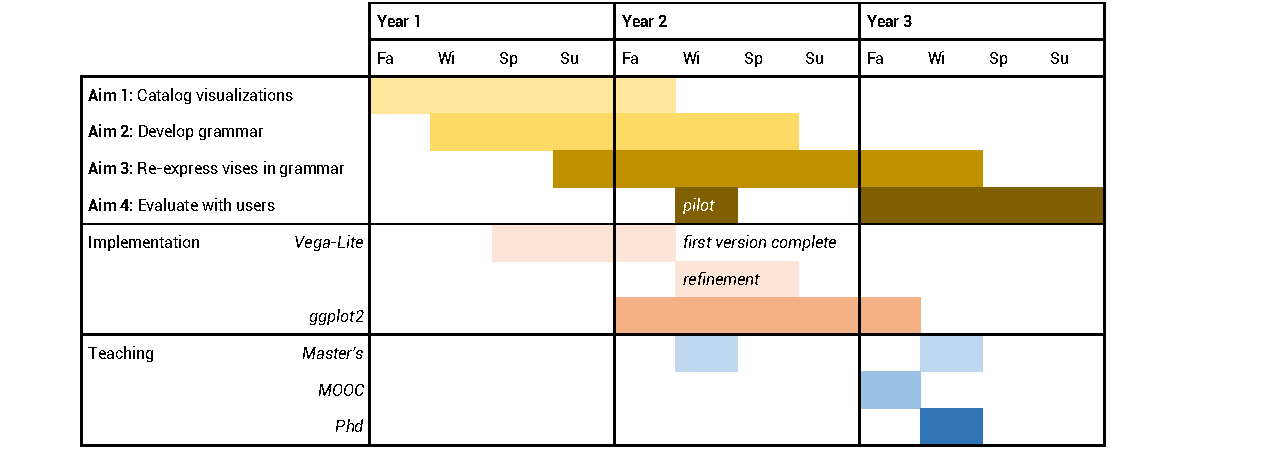
\includegraphics[width=\columnwidth]{img/timeline}

\noindent The first implementation of the grammar will be created on top of Vega-Lite, and timed to have a first version completed just before I teach the Master's-level visualization class in the beginning of Winter of the second year of the project. This will allow me to teach the grammar to students (who will already be learning Vega-Lite anyway), and continue refining both the grammar and the implementation. This first teaching run-through will also be an opportunity to pilot studies for Aim 4, giving advance testing and time to work out bugs before testing the system in a controlled study for Aim 4 in the third year of the project. For participants in the evaluation studies, I will recruit students from the Master's course I teach in Year 3, in which students will be taught the grammar of graphics.

\section{Broader Impacts of the Proposed Work}

\noindent This work has several broader impacts:

\noindent\textbf{Societal Outcomes, Toolkits:}
This work has the potential to make the production of effective uncertainty visualizations easier and more widespread, improving the communication of uncertainty and risk across a range of domains. If toolkits developed in this work are adopted by data journalists, improving their uncertainty communication, the ability of audiences to understand and act upon uncertainty in news reports will be improved. This has wide-reaching implications for data journalism that impacts everyday decision-making, from election outcomes to forecasts of extreme weather events, such as floods or hurricanes. Better uncertainty visualization toolkits integrated into statistical modeling workflows (such as R, ggplot2 \cite{wickham2016ggplot2}, and tidybayes \cite{kay2017tidybayes}) would raise standards of scientific communication, ultimately improving the way that scientists and laypeople interpret and act upon the results of research across a range of domains.

\noindent\textbf{Publications:}
Besides instantiating the results of this work in freely-available, open source toolkits, I will publish results in scholarly conferences and journals, such as the InfoVis track of the IEEE VIS Conference, where accepted papers appear in the IEEE journal Transactions in Visualization and Computer Graphics (TVCG). I also publish in the ACM SIGCHI Conference on Human Factors in Computing systems, the premier venue in Human-Computer Interaction. I have a track record of publishing in both venues.

\section{Investigator Qualifications}
\noindent I have substantial experience in the development and controlled evaluation of uncertainty visualizations (\eg \cite{Fernandes2018, kay2016bus, kale2018hypothetical, hullman2018pursuit, hullman2018imagining, greis2017uncertaintyhci}). In addition, I have published two open source R packages \cite{kay2016artool, kay2017tidybayes} on the Comprehensive R Archive Network (CRAN) \cite{hornik2012cran}, which entails following strict package development standards \cite{hornik2012cran, cran1999writing}, gaining the approval of archive maintainers, and being responsive to package maintenance issues in order to maintain status in the archive. The tidybayes \cite{kay2017tidybayes} package, in particular, represents my initial work at integrating Bayesian statistical analysis into a grammar of graphics workflow, and currently garners approximately 1000 downloads per month. My background positions me well both to create a formal description of uncertainty visualization within the grammar of graphics, and to build and deploy toolkits implementing this vision that have the potential to be adopted more widely.

\section{Results of Prior NSF Support}
\noindent Dr. Kay is a PI on NSF grant IIS 1815790: CHS: Small: Collaborative Research: Validating and Communicating Model-based 
Approaches for Data Visualization Ability Assessment (\$238,848; 09/01/2018--08/31/2021).  This project uses studies of visualization effectiveness to inform our understanding of the abilities and biases of viewers, both individually and collectively. \textbf{Intellectual Merit}: Using a combination of experiments, statistical modeling, and interview studies, this work challenges long-standing assumptions about visualization effectiveness, and will lay a foundation for future experiments that account for differences in visualization reading ability. \textbf{Broader Impact}: This work will support a broader educational goal of using robust statistical modeling techniques in experimentation, through course modules that can be integrated into existing data visualization courses, and through outreach activities that allow individuals to see how well they perform visualization tasks compared to others who have taken the experiments. As this project was recently funded, no publications have yet resulted from it.


\pagebreak
\pagebreak


\section{OLD TEXT}





Following this experiment, the grammar may be refined based on qualitative feedback.




To determine whether or not the probabilistic grammar of graphics is able to better support the construction


could happen, which would lead to more confusion than insights. More broadly, creating uncertainty visualizations is a difficult because of the lack of supporting formalism and tools. 

for an example, see Section XXX). I will also conduct a user study to assess whether or not visualization authors can rapidly and correctly uncertainty visualizations, by asking experienced visualization authors to create visualizations of particular distributions / uncertainties using both the visualization uncertainty grammar and an existing implementation of the grammar of graphics (e.g., ggplot2 or Vega-Lite).


; partly, this will be achieved through grounding the grammar in the specification of probability distributions, such that if an author wishes to (say) communicate a particular conditional probability, they would specify this in the grammar and the visualization system would determine how to do that. This will allow authors to easily swap out and explore different presentations while maintaining the correctness of the output visualizations.



Despite the importance of conveying uncertainty, creating effective uncertainty visualizations is difficult and error-prone in practice. The New York Times election needle, while employing an effective technique, was a bespoke JavaScript website created by one of a small number of premier data journalism outfits. For effective uncertainty visualization to flourish, visualization designers without access to a dedicated visualization programming team should be able to create sophisticated, correct, highly effective uncertainty visualizations within toolkits they are familiar with.



Recently, the \textit{New York Times} used a chart to show the relationship between income mobility and race \cite{emily_badger_income_2018}; one part of the visualization encodes $P(Race \vert Adult\ Income)$, ``the probability of me being black given I'm a rich adult''. A reader of this article might care about a more meaningful conditional, $P({Adult\ Income \vert Race })$, \textit{i.e.}, ``the probability of me ending up as a rich adult given I'm black''. 




\begin{itemize}
    \item expanded and instantiated the grammar of graphics in different applications areas and programming environments \cite{Park2017,Satyanarayan2017vegalite, Wickham2010layered_grammar, yin_ggbio_2012} % ATOM, vega-lite, ggplot, (this random genomic visualization thing)
    \item These examples do not have a notion of probability distributions and consequently, mapping uncertainty information to visual elements could be cumbersome.
\end{itemize}

- technical complexity of creating and prototyping effective uncertainty visualization is high --- involves probability distributions, sampling, animation, etc. E.g. NYT needle --- needs to deal with sampling, mapping that onto states of the animation, setting up animation, updating uncertainty, etc. All these aspects of the visualization as specified are intermingled, prototyping a new animated visualization of uncertainty is difficult --- can't just change the representation and have it all still work, would need to rewrite how the whole thing works. Add on top of that the difficulty people have in understanding things like conditional probability, and different prototypes are hard to get right. 




As a consequence, the existing uncertainty visualizations are created on a case-by-case basis. (New York Time's HOPs about jobs added \cite{neil_irwin_how_2014}



(Conclude with the benefits of having a grammar)

However, these existing formalisms don’t afford the same convenience when the user wants to create uncertainty visualizations. (Some limitations in \cite{Wickham2010layered_grammar})

One of the obstacles is that probability distributions are difficult to reason with and existing instantiations of grammar of graphics, (\texttt{ggplot} has \texttt{stat} things) do not directly support input data as statistical objects such as distributions. This gap leads to (compared to creating ``normal'' visualizations) lower correctness and ease of use.

Product plots and limitations of it \cite{wickham_product_2011} (future work)


Would like to combine the power of the grammar and the need to facilitate uncertainty communication in journalism, scientific communities, and beyond.







\noindent \textbf{Custom/generated uncertainty visualizations}:



\begin{itemize}
    \item An uncertainty visualization is defined as 
    \item Using discrete elements as samples of the underlying distribution \cite{kay2016bus, park2016gatherplots, Park2017}
    \item Using color properties to encode uncertainty \cite{lucchesi_visualizing_2017, Correll2018}
    \item Geospatial data \cite{lucchesi_visualizing_2017, liu2018visualizing}
    \item Using area/lengths/outlines to show proportions \cite{wickham_product_2011, Gortler2018}
    \item Animated \cite{hullman2015hops}
    \item Problem: one-off, difficult to 
\end{itemize}






uncertainty vis, \cite{kale2018hypothetical} \cite{kay2016bus, Fernandes2018}

tidybayes






% x grammar of graphics, 
% x ggplot, 
% x vega-lite, 
% x product plots, 
% x unit grammar, 
% x gather plots


\newpage
\setcounter{page}{1}
\section*{References}
References to the work of the PI are indicated with an \emph{m}.

\bibliographystylem{abbrv}
\nocitem{*}
\bibliographym{bib/ours}
%\begin{btSect}{bib/ours}
%\renewcommand{\bibprefix}{*}
%\section*{References to our work}
%\btPrintCited
%\end{btSect}

\bibliographystyle{abbrv}
\bibliography{bib/others}
%\begin{btSect}{bib/others}
%\renewcommand{\bibprefix}{}
%\section*{Other References}
%\btPrintCited
%\end{btSect}

\end{document}
